\section{Evaluation}


Why does text longevity not do so well as edit longevity?
As part of our investigation, we started looking at specific
instances of text longevity values.
In Figures~\ref{fig:ts-GeorgeWBush} and~\ref{fig:ts-SantaCruzBeachBoardwalk},
we see the text survival for two different contributions;
both do seem to have the general ``exponential'' shape
that we previously described.
Also computed in each figure is the text longevity metric based on
the 20~revisions shown in each graph, but notice that the text
longevity computed for
Figure~\ref{fig:ts-GeorgeWBush} doesn't exhibit curve we expect.

\begin{figure}[tbph]
\centering
\framebox{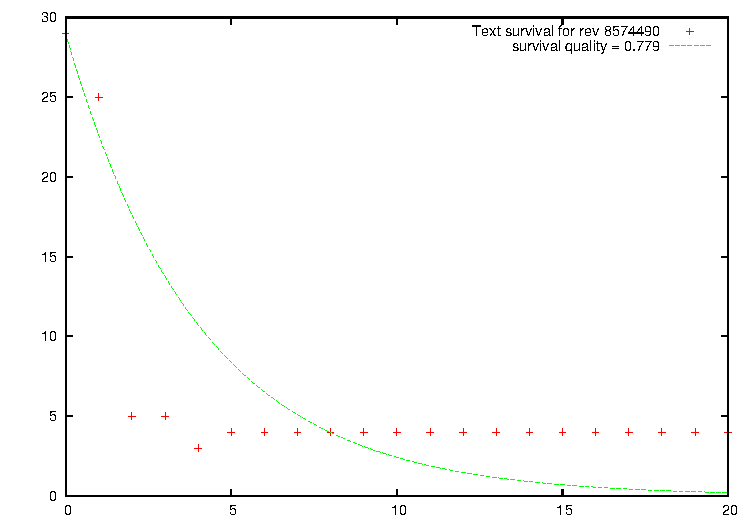
\includegraphics[width=0.8\textwidth]{part-F70-editquality/graph-TS-GeorgeWBush-8574490}}
\caption{The text survival graph for the text contributed early
        in the history of article \textit{George W.~Bush}.
	The graph also shows the text survival quality
	computed based on 20~revisions.
	}
\label{fig:ts-GeorgeWBush}
\end{figure}

\begin{figure}[tbph]
\centering
\framebox{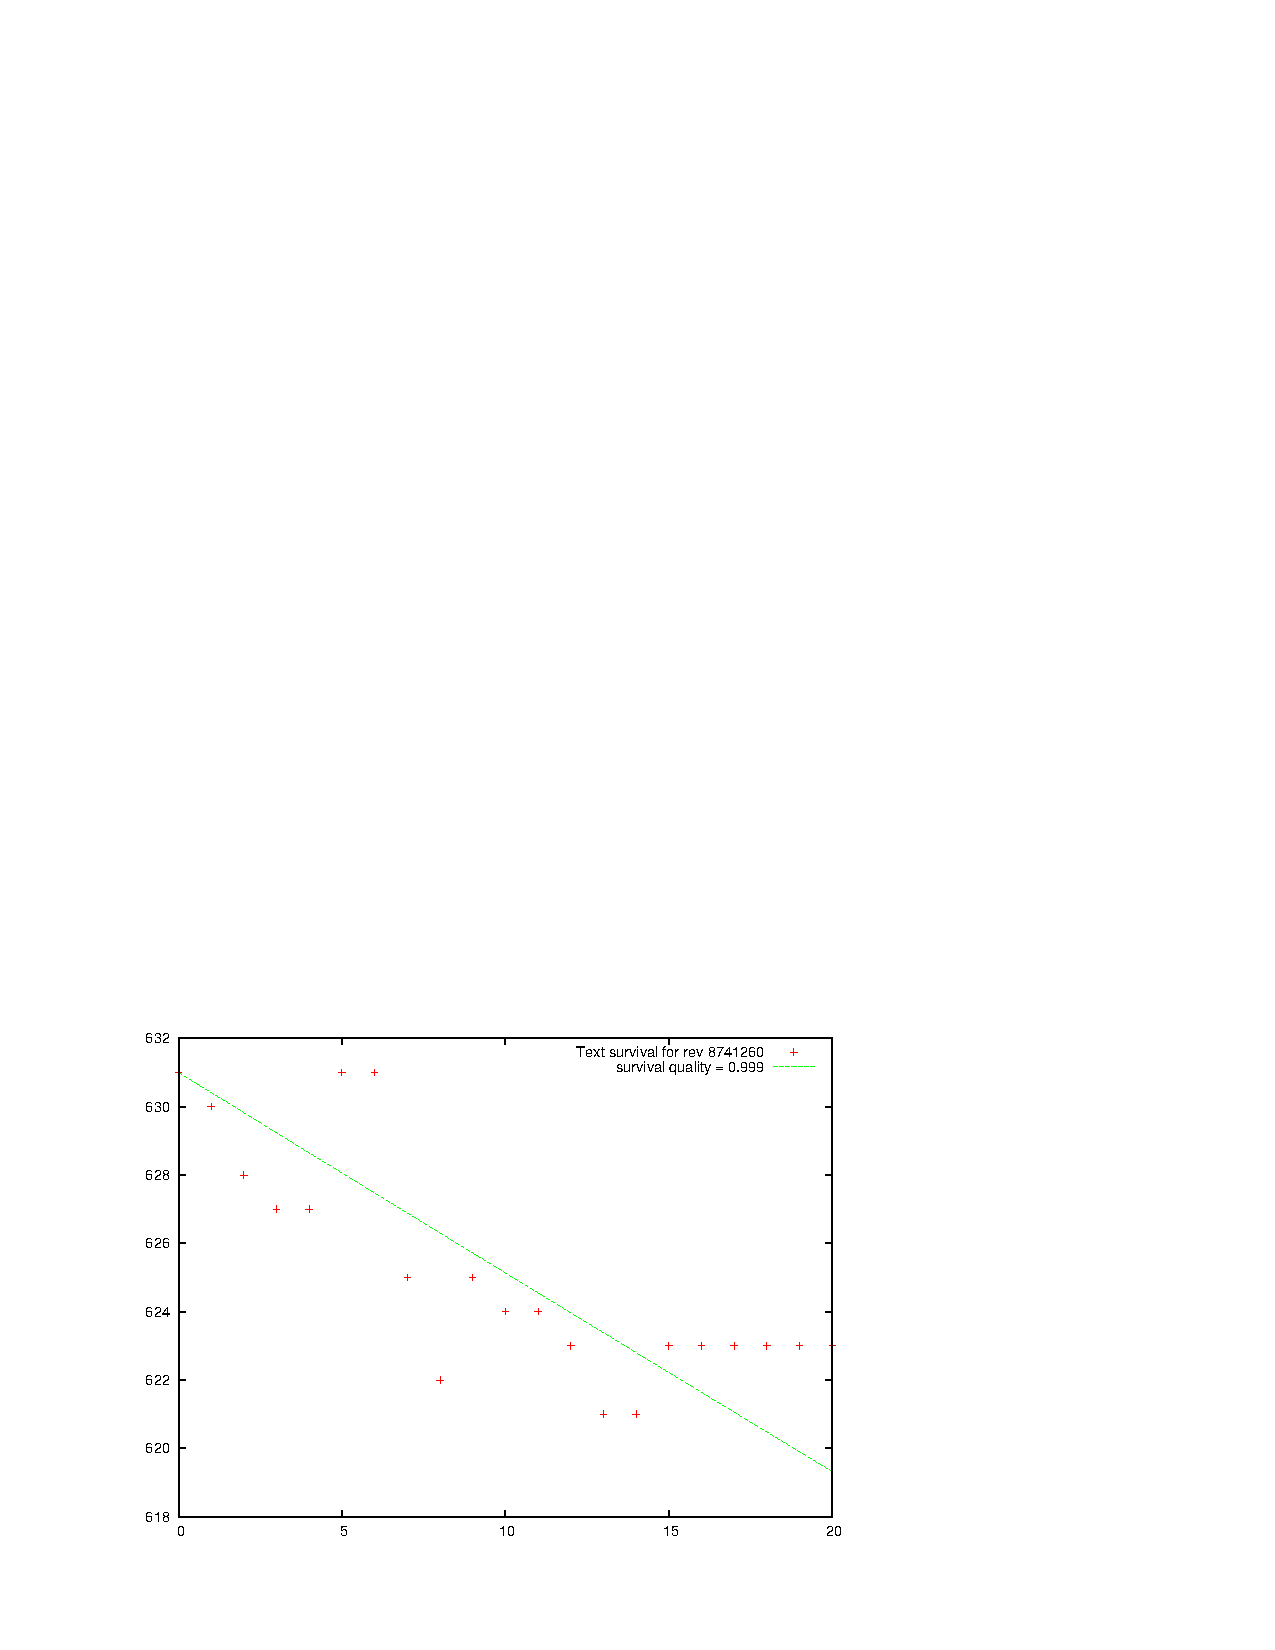
\includegraphics[width=0.8\textwidth]{part-F70-editquality/graph-TS-SantaCruzBeachBoardwalk}}
\caption{The text survival graph for the text initially contributed
	as part of the article \textit{Santa Cruz Beach Boardwalk}.
	The majority of the editing to the contributed text happens
	in the next few revisions, before the text stabilizes.
	The graph also shows the text survival quality
	computed based on 20~revisions.
	}
\label{fig:ts-SantaCruzBeachBoardwalk}
\end{figure}

The explanation for this discrepancy turns out to be a flaw in our
thinking about the original model.
While the text survival for contributions does seem to have an
exponential look to it, exponentials do not approach some fixed
non-zero value --- they approach zero.
In order to fit the curve we are describing, the last value
(in the case of the data shown in Figure~\ref{fig:ts-GeorgeWBush},
the amount of text that survives after the $20^{th}$ revision)
should be taken as the ``zero reference point'' which is subtracted
from all the values.
Applying our exponential curve fitting technique to these new values
will give a much better approximation to the data.
The problem with this better fit is that it changes the meaning of
a score of zero; instead of meaning that the text was immediately deleted,
a score of zero would mean that the text immediately reached its
final survival level.
In other words, we would be measuring how quickly the text stabilizes,
rather than how much agreement there was that the text belonged in
the article.

